\thispagestyle{empty}
\begin{center}
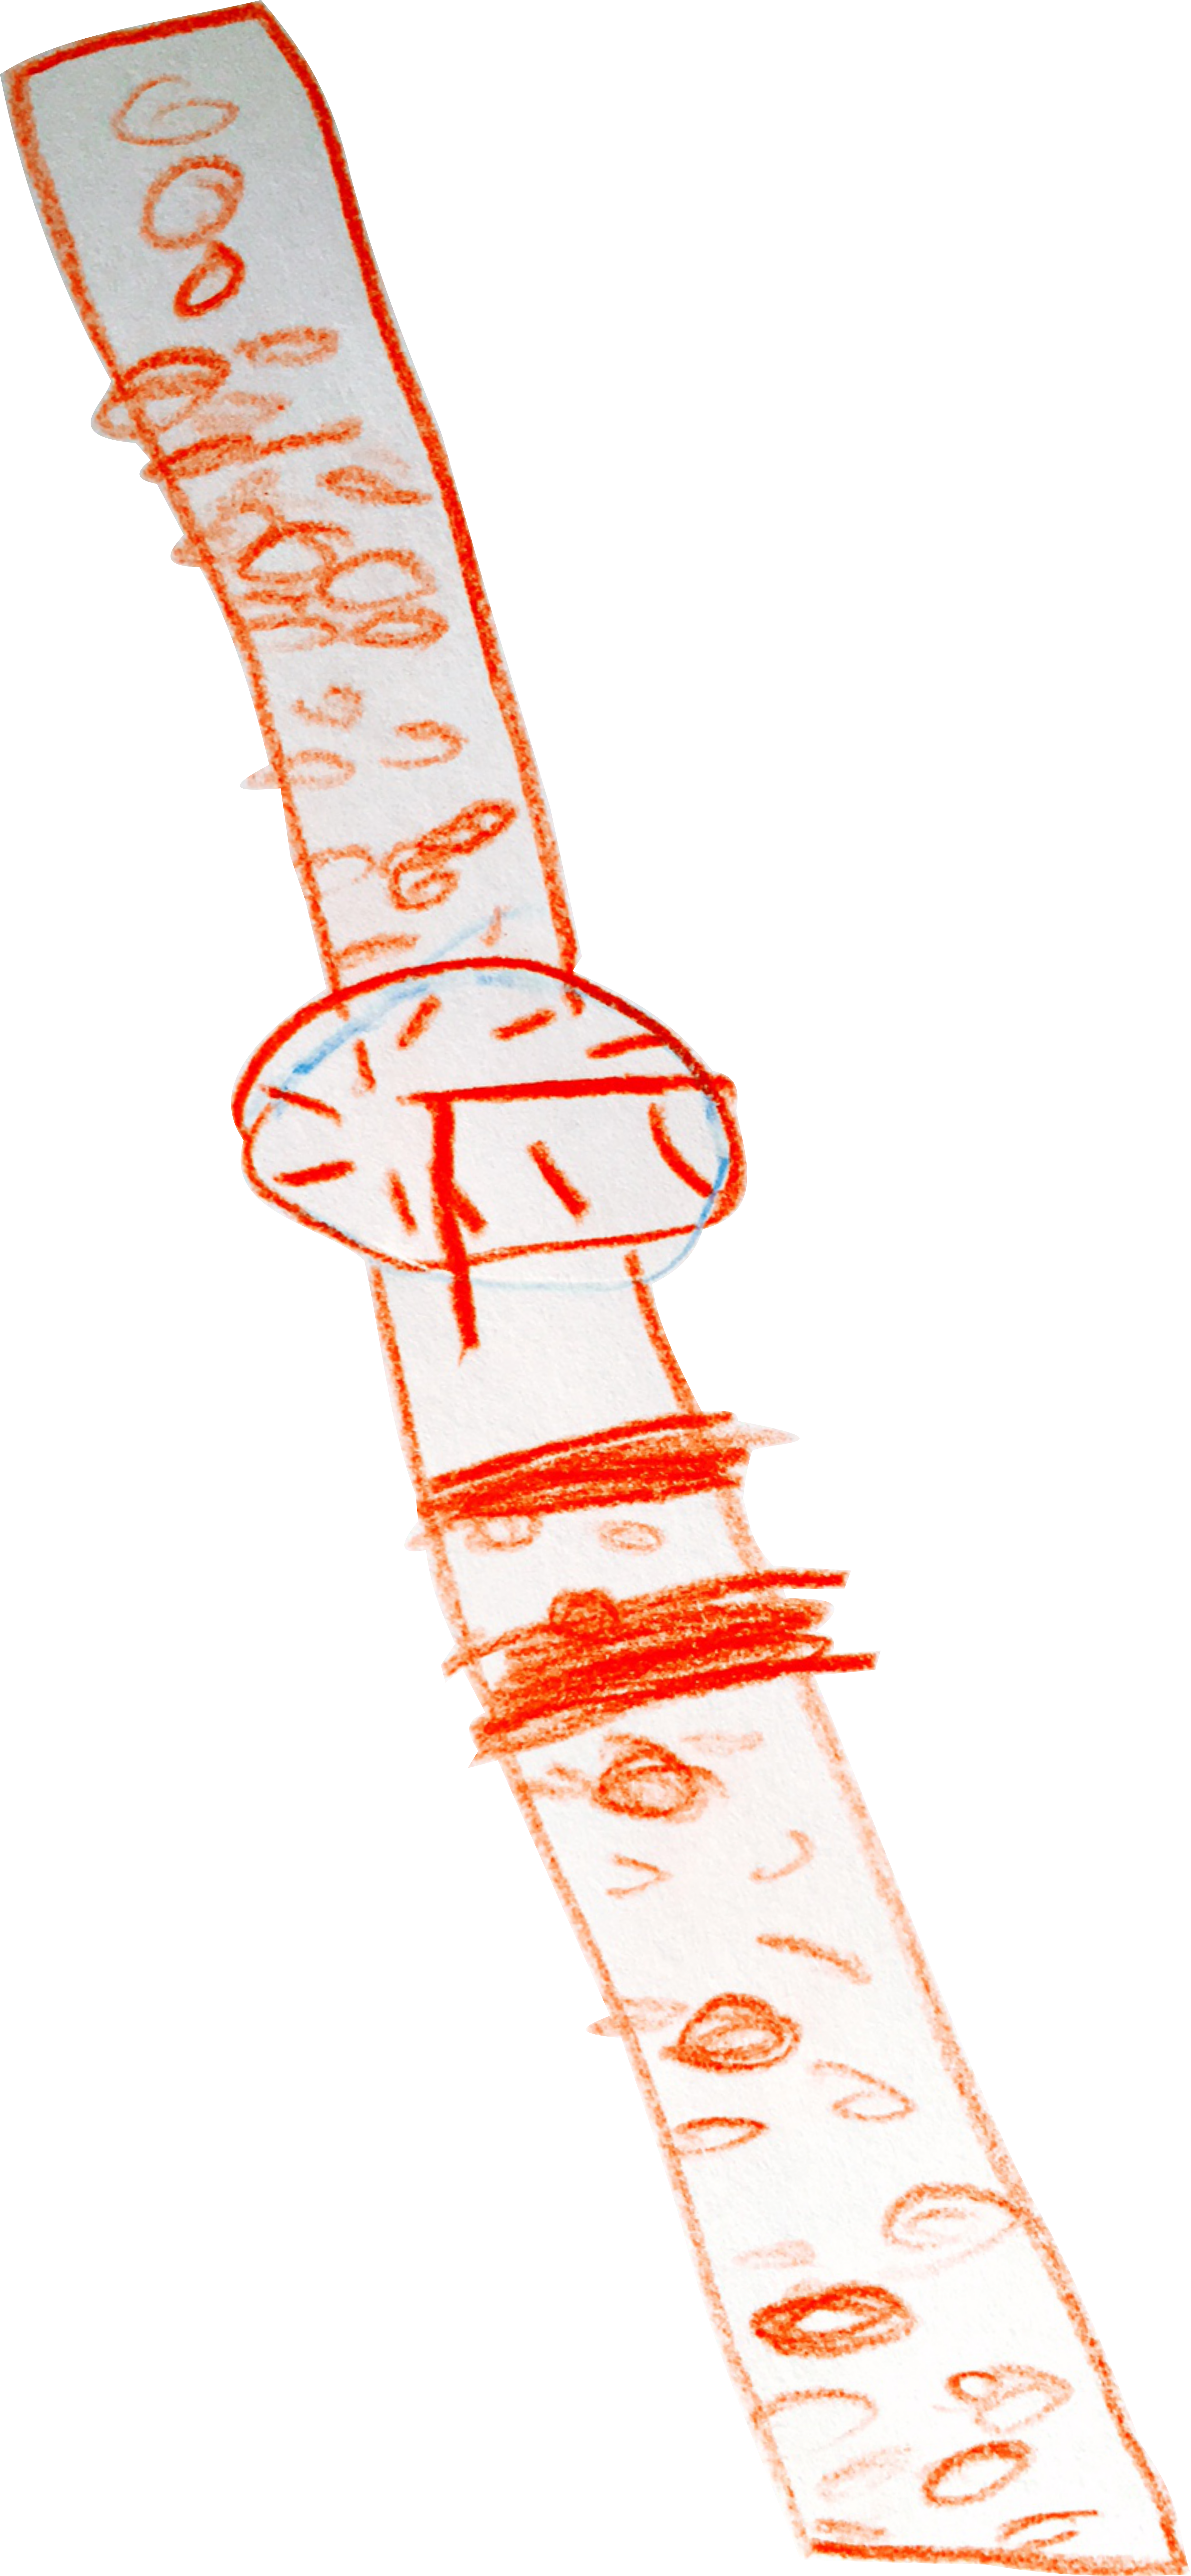
\includegraphics[height=.8\textheight]{./bilder/160120_uhr.png}
\end{center}
\vskip 2cm
{\Huge\color{farbe}\hfill{\ttfamily{Der rosarote Elefant}}}
\addcontentsline{toc}{chapter}{}
\newpage
%%%%%%%%%%%%%%%%%%%%%%%%%%%%%%%%%%%%%%%%%%%%%%%%%%%%%%%%%%%%%%%%%%%%%%%%%%%%%%%
\lettrine[lines=2, lhang=.2, loversize=.25, lraise=0.05, findent=0.1em,
nindent=0em]{L}{uca} der Elefant war von der Herde ausgestossen worden, weil er rosarot war. Sein Freund war Ben und der war eine Maus. Luca sagte zu Ben:

\enquote{Wir müssen etwas unternehmen, ich will nicht die ganze Zeit von der Herde ausgestossen sein.}

Ben sagte: \enquote{Ich muss mir etwas üblergenen -- Ich habe eine Idee: Wir könnten den grauen Stoff, den die Menschen überall verteilen, nehmen, und auf Dich kleben!}

Und genau das haben die beiden auch gleich gemacht. Sie haben den grauen Stoff gesammelt, den die Menschen in der Natur verteilt haben und haben ihn aufgeklebt. Aber leider hat es immer noch Lücken gegeben. Am Rüssel und an den Schultern ist der Stoff nicht zusammen gekommen. 

Dann geht Luca zu seiner Herde uns sagt: 

\enquote{Ich bin jetzt grau!}

Aber die anderen Elefanten lachen ihn aus: 

\enquote{Du hast ja nur Stoff angeklebt!}

Und deswegen sagt Luca zu Ben, nachdem sie den Stoff wieder abgemacht haben:

\enquote{Ich bin immer noch pink, was soll ich nur machen?}

\enquote{Es gibt doch so graue Farbe, mit der kannst du dich anstrreichen, dann bist du grau!}

Der Elefant antwortet Ben:

\enquote{Aber ich komme doch gar nicht bis unter meinen Bauch mit meinem Rüssel und du kannst nicht so hoch klettern!}

Ben sagt:

\enquote{Ich habe andere Mäuse als Freund, wir können einen Stapel machen.}

Dannach kommen alle Mäuse und machen einen Stapel und malen Luca an. Und dann geht Luca zu der Herde, aber die graue Farbe tropft und rutscht herunter. Und sie sagen:

\enquote{Du bist immer noch pink, Du bist immer noch pink, Du bist immer noch pink!}

Dan nsagt aber die Familie von Luca:

\enquote{Es ist egal, wenn Luca pink ist, er ist ja immer noch eon Elefant!}

Darauf sagen die anderen Elefanten:

\enquotr{Mach das komische graue Gekleckse weg und dann bist du wieder ein richtiger Elefant!}

ENDE
